%%% Copyright (C) 2021 Vincent Goulet
%%%
%%% Ce fichier fait partie du projet
%%% «Programmer avec R»
%%% https://gitlab.com/vigou3/programmer-avec-r
%%%
%%% Cette création est mise à disposition sous licence
%%% Attribution-Partage dans les mêmes conditions 4.0
%%% International de Creative Commons.
%%% https://creativecommons.org/licenses/by-sa/4.0/

\chapter{Algorithmes et algorithmique}
\label{chap:algorithmes}

\def\scriptfilename{\currfilebase.R}

\begin{objectifs}
\item Résoudre un problème sous la forme d'un algorithme en langage
  naturel ou en pseudocode.
\item Utiliser des instructions conditionnelles dans un algorithme.
\item Utiliser la récursion et l'itération pour effectuer des tâches
  répétitives dans un algorithme.
\item Évaluer la performance d'un algorithme à l'aide de la notation
  $O()$.
\end{objectifs}

Marianne et Alexandre doivent fournir une solution logicielle à un
problème donné. Sitôt la lecture de l'énoncé du problème complétée,
ils se précipitent sur le clavier pour coder leur solution. Rapidement
bloqués, pensant qu'ils butent sur un problème de syntaxe ou
d'utilisation d'une fonction, ils demandent de l'aide. Lorsqu'on leur
demande qu'est-ce qu'ils essaient de faire, quelle est la nature de leur
solution, ils ne peuvent répondre que par un long silence.

Dans mon rôle de professeur, j'ai été témoin de la scène ci-dessus à
de nombreuses reprises. Marianne et Alexandre font une erreur commune
chez les programmeurs --- et pas que chez les débutants: commencer à
coder sans avoir au préalable suffisamment réfléchi à la solution. Il
leur manque un plan clair des étapes à suivre pour résoudre le
problème. Or, ce plan, ou la recette à suivre pour transformer les
entrants d'un problème en une solution, c'est
l'\index{algorithme}\emph{algorithme}. Travailler sans algorithme,
c'est comme naviguer sans boussole.

Puisque programmer requiert des algorithmes, l'étude de la
programmation doit par conséquent s'accompagner de notions
d'\index{algorithmique}\emph{algorithmique}, la science qui étudie les
algorithmes et les structures de données. L'algorithmique est une
discipline riche en techniques ingénieuses et en analyses
mathématiques poussées. Connaitre ses principes de base et étudier
certains algorithmes classiques vous permettra de mieux planifier vos
méthodes de résolution de problème. En effet, un bon algorithme permet
de résoudre en quelques secondes un problème qui pourrait autrement
prendre des années.

L'étude des algorithmes s'accompagne habituellement de celle des
structures de données ou, en d'autres termes, de la manière
d'organiser les données dans un ordinateur. Comme nous le verrons au
\autoref{chap:donnees}, il existe bien différentes structures de
données en R, mais leur réelle mise en œuvre demeure tout à fait
transparente pour les programmeuses et les programmeurs. C'est
pourquoi nous ferons l'impasse sur des notions que l'on retrouve dans
tous les ouvrages classiques d'algorithmique, comme le tableau
(\emph{array}), la liste chainée (\emph{list}), l'arbre (\emph{tree})
ou la table de hachage (\emph{hashtable}).

Le présent chapitre est inspiré de \citet{Sussman:scheme:1996},
\citet{Knuth:ACP:vol1:1997} et \citet{Stephens:algorithms:2013}.


\section{Définition et analogie}
\label{sec:algorithmes:definition}

Un \index{algorithme}algorithme est une procédure de calcul
permettant de résoudre un problème bien spécifié. L'algorithme
explique, de manière non ambigüe et dans un nombre d'opérations fini,
comment, à partir d'entrants, obtenir l'extrant solution du problème.

Pour se mériter un algorithme, un problème doit renfermer une dose
minimale de complexité: personne n'écrit un algorithme pour extraire
le quatrième élément d'un vecteur de données. On suppose que cela fait
partie de la définition de vecteur et que vous savez comment effectuer
l'opération dès lors que vous connaissez le langage de programmation
sous-jacent.

Dans la même veine, un algorithme ne dépend pas du langage de
programmation employé, car il fournit les étapes pour résoudre un
problème, non pas leur mise en œuvre. En d'autres termes, un
algorithme explique \emph{ce qu'il faut faire} pour résoudre un
problème et non \emph{comment le faire}.

Illustrons le concept d'algorithme par l'un de ses plus illustres
représentants: l'\Index{Euclide@Euclide (algorithme)}algorithme
d'Euclide (c.~300 av. J.-C.), une procédure de calcul du plus grand
commun diviseur (PGCD) de deux nombres entiers $m$ et $n$. Selon
\citet{Knuth:ACP:vol2:1997}, il s'agirait de l'un des plus anciens
algorithmes. Il repose sur l'idée que le PGCD de $m$ et $n$ est aussi
le PGCD de $n$ et du reste de la division de $m$ par $n$.

\begin{algorithme}[Algorithme d'Euclide]
  \label{algo:algorithmes:euclide}
  Calculer le plus grand commun diviseur de deux entiers positifs $m$
  et $n$ avec, sans perte de généralité, $n < m$.
  \begin{enumerate}
  \item Diviser $m$ par $n$ et poser $r$ égal au reste de la division.
    (Nous avons alors $0 \leq r < n$.)
  \item Si $r = 0$, retourner la valeur $n$.
  \item Poser $m \leftarrow n$, $n \leftarrow r$, puis retourner à
    l'étape 1.
  \end{enumerate}
\end{algorithme}

Suivons les étapes de l'\index{Euclide@Euclide (algorithme)}algorithme
d'Euclide avec $m = 544$ et $n = 119$. À l'étape~1, nous déterminons
que $544/119 = 4 + 68/119$, donc nous posons $r \leftarrow 68$.
Puisque $r \neq 0$, l'étape~2 de l'algorithme ne s'applique pas. Nous
passons donc à l'étape~3 et nous posons $m \leftarrow 119$ et
$n \leftarrow 68$. De retour à l'étape~1, nous déterminons cette fois
que $r \leftarrow 51$, ce qui mène encore à l'étape~3 et
$m \leftarrow 68$ et $n \leftarrow 51$. Après un autre cycle, nous en
sommes à $m \leftarrow 51$ et $n \leftarrow 17$. Cette fois, nous
posons $r \leftarrow 0$ à l'étape~1 et la procédure s'arrête ensuite à
l'étape~2. Le plus grand commun diviseur de $544$ et $119$ est $17$.
Le \autoref{tab:algorithmes:euclide} dresse le sommaire des opérations
ci-dessus.

\begin{table}
  \centering
  \caption{Calcul du plus grand commun diviseur de $544$ et $119$ avec
    l'algorithme d'Euclide}
  \label{tab:algorithmes:euclide}
  \begin{tabular}{crrr}
    \toprule
    \text{Étape} & $m$ & $n$ & $r$ \\
    \midrule
    $1$ & $544$ & $119$ & $68$ \\
    $3$ & $119$ & $ 68$ & $68$ \\
    $1$ & $119$ & $ 68$ & $51$ \\
    $3$ & $ 68$ & $ 51$ & $51$ \\
    $1$ & $ 51$ & $ 17$ & $ 0$ \\
    $2$ &   --- & $ 17$ &  --- \\
    \bottomrule
  \end{tabular}
\end{table}

\warningbox{L'ordre des opérations à l'étape~3 de
  l'\autoref{algo:algorithmes:euclide} est important. En effet,
  l'action «Poser $m \leftarrow n$, $n \leftarrow r$» est très
  différente de «Poser $n \leftarrow r$, $m \leftarrow n$» puisque
  dans cette dernière, la valeur de $n$ est perdue après la première
  réaffectation. La seconde action est équivalente à «Poser
  $n \leftarrow r$, $m \leftarrow r$».}

Selon \citet[section~1.1]{Knuth:ACP:vol1:1997}, un algorithme devrait
réunir cinq caractéristiques.\footnote{%
  Liste adaptée de la version française fournie par
  \citet{Wikipedia:Algorithme}.}
\begin{enumerate}
\item \emph{Finitude}. Un algorithme doit toujours se terminer après
  un nombre fini d’étapes. Ce nombre peut toutefois devenir très
  grand.
\item \emph{Définition précise}. Chaque étape d'un algorithme doit
  être définie précisément; les actions à réaliser doivent être
  spécifiées rigoureusement et sans ambigüité pour chaque cas.
\item \emph{Entrées}. Un algorithme comporte aucune, une ou plusieurs
  \emph{entrées}, des quantités fournies à l'algorithme avant qu'il ne
  commence ou qui sont allouées dynamiquement durant son exécution.
  Ces entrées proviennent d'un ensemble d'objets bien spécifié. Par
  exemple, l'\autoref{algo:algorithmes:euclide} comporte deux entrées,
  les nombres $m$ et $n$, provenant de l'ensemble des entiers
  positifs.
\item \emph{Sorties}. Un algorithme comporte une ou plusieurs
  \emph{sorties}: des quantités ayant une relation spécifiée avec les
  entrées. L'\autoref{algo:algorithmes:euclide} a une seule sortie,
  soit la valeur $n$ de l'étape~2, le plus grand commun diviseur des
  entrées.
\item \emph{Efficacité}. On s'attend généralement d'un algorithme
  qu'il soit \emph{efficace} dans le sens où toutes les opérations
  qu'il doit accomplir sont suffisamment élémentaires pour pouvoir
  être en principe réalisées dans une durée finie par une personne
  munie de papier et d'un crayon.
\end{enumerate}

Pour bien comprendre la nature et la portée d'un algorithme, il est
assez utile de le comparer à une recette de cuisine. Dans une recette,
les entrées sont les ingrédients, la procédure les diverses étapes et
la sortie, le plat préparé.

Comme un algorithme, une recette repose sur un certain nombre
d'instructions élémentaires qui se passent d'explication, comme
saisir, mijoter, mélanger, etc. La recette est aussi indépendante des
ustensiles utilisés comme l'algorithme l'est du langage de
programmation.

Surtout, surtout, une recette explique les étapes à suivre pour
obtenir le plat voulu, mais, sauf peut-être pour certaines opérations
plus délicates, elle n'explique pas \emph{comment} réaliser chaque
étape. S'il faut ajouter du lait dans un mélange à gâteau, la recette
n'indique pas de sortir le lait du réfrigérateur, de vérifier la date
de péremption et de verser le lait dans la tasse à mesurer jusqu'à la
ligne correspondant à la quantité voulue! Un algorithme ne contient pas
plus d'instructions pour vérifier la validité des entrées ou pour
effectuer des opérations de base comme les opérations arithmétiques,
la lecture de données, l'indiçage d'un vecteur, etc.

En revanche, on s'attend généralement d'un algorithme, qui est destiné
à un ordinateur, qu'il soit plus précis qu'une recette. En effet, un
ordinateur éprouverait beaucoup de difficulté avec une instruction
comme «saler et poivrer au gout»!

\tipbox{C'est une erreur commune dans la rédaction d'un algorithme de
  fournir des détails de mise en œuvre superflus, de surcroit dans un
  langage de programmation bien précis. Lorsque vous écrirez un
  algorithme, demandez-vous si vous êtes en train d'expliquer comment
  mesurer une quantité de lait avec une tasse à mesurer de marque
  ACME.}


\section{Pseudocode}
\label{sec:algorithmes:pseudocode}

Puisqu'il s'agissait du premier exemple d'algorithme complet, j'ai
choisi de présenter l'\autoref{algo:algorithmes:euclide} dans un
format très près du langage naturel.

Une autre manière très populaire d'exprimer les algorithmes consiste à
utiliser du \index{pseudocode}\emph{pseudocode}, un «langage»
similaire à un langage de programmation, mais toujours sans référence
à un langage en particulier. L'écriture en pseudocode permet parfois
de mieux prendre la mesure de la structure et des détails d'un
algorithme avant d'en attaquer la mise en œuvre.

Voici de nouveau l'\index{Euclide@Euclide (algorithme)}algorithme
d'Euclide, présenté cette fois en pseudocode. Portez-y une attention
toute particulière puisqu'il ne s'agit pas d'une transcription directe
de l'\autoref{algo:algorithmes:euclide}. Vérifiez que les deux
versions de l'algorithme retournent bien le même résultat.

\begin{algorithme}[Algorithme d'Euclide, version en pseudocode]
  \label{algo:algorithmes:euclide:pseudo}
  Calculer le plus grand commun diviseur de deux entiers positifs $m$
  et $n$ avec, sans perte de généralité, $n < m$.
\begin{Schunk}
\begin{Verbatim}[commandchars=\\\{\}]
PGCD(entier m, entier n)
  Tant que (n \neq 0)
    r \leftarrow m mod n
    m \leftarrow n
    n \leftarrow r
  Fin Tant que
  Retourner m
Fin PGCD
\end{Verbatim}
\end{Schunk}
\end{algorithme}

\tipbox{L'opération \index{modulo}modulo, notée en mathématiques
  $m \mod n$, représente le reste de la division de $m$ par $n$. Par
  exemple, tel que calculé précédemment, $544 \mod 119 = 68$.}

Il n'existe pas réellement de normes de composition pour le
pseudocode. L'\autoref{algo:algorithmes:euclide:pseudo} reprend
toutefois quelques-unes des conventions les plus usuelles.

La procédure de calcul faisant l'objet de l'algorithme est rédigée
sous forme d'une fonction\footnote{%
  C'est la terminologie de R. Une unité de code qui effectue un
  traitement donné porte divers noms selon le langage de
  programmation: fonction, routine, sous-routine, méthode, procédure,
  sous-procédure\dots}. %
L'algorithme débute par la \index{signature}\emph{signature} de la
fonction (son nom avec le nom et le type de tous les arguments). Le
code est \index{indentation}indenté (décalé vers la droite) après la
signature de la fonction pour montrer qu'il fait partie du corps de la
fonction.

Le bloc délimité par les instructions \code{Tant que
  (\meta{condition})} et \code{Fin Tant que} forme une
\index{boucle}\emph{boucle} dont le contenu --- lui aussi indenté ---
est exécuté tant et aussi longtemps que la \meta{condition} est vraie.

L'instruction \code{Retourner} met immédiatement fin à la fonction,
ici en retournant la valeur \code{m}.

Enfin, on présente le pseudocode comme du code informatique dans une
police non proportionnelle qui préserve l'alignement vertical des
caractères.


\section{Évaluation conditionnelle}
\label{sec:algorithmes:if-else}

Plusieurs algorithmes, même les plus simples, nécessitent de pouvoir
effectuer des opérations différentes selon le résultat d'un test. Par
exemple, pour effectuer le banal calcul de la valeur absolue d'un
nombre, nous devons vérifier si le nombre est positif, négatif ou nul
pour retourner un résultat différent en fonction de la règle suivante:
\begin{equation*}
  \lvert x \rvert =
  \begin{cases}
    x, & \text{si } x > 0 \\
    0, & \text{si } x = 0 \\
    -x, & \text{si } x < 0.
  \end{cases}
\end{equation*}

De telles constructions requièrent des \emph{instructions
  conditionnelles} qui permettent d'effectuer différents calculs selon
le résultat d'une condition booléenne (vraie ou fausse). Il en existe
quatre grands types.

\begin{itemize}
\item Les instructions conditionnelles à un volet de la forme
  \begin{quote}
    Si \meta{condition}, alors \meta{conséquence}
  \end{quote}
  Dans cette construction, la \meta{conséquence} est évaluée seulement
  lorsque la \meta{condition} est vraie. Dans le cas contraire, il ne
  se passe rien et le déroulement de l'algorithme se poursuit
  normalement. Nous avons utilisé une telle instruction conditionnelle
  à l'étape~2 de l'\autoref{algo:algorithmes:euclide}. La locution
  «alors» est souvent omise dans les algorithmes comme, d'ailleurs,
  dans la syntaxe de plusieurs langages de programmation.
\item Les instructions conditionnelles à deux volets de la forme
  \begin{quote}
    Si \meta{condition}, alors \meta{conséquence}, \\
    sinon \meta{alternative}
  \end{quote}
  Cette construction permet d'effectuer un choix entre deux actions:
  ou bien la \meta{condition} est vraie et la \meta{conséquence} est
  évaluée, ou bien la \meta{condition} est fausse et c'est alors
  l'\meta{alternative} qui est évaluée. Le déroulement de l'algorithme
  se poursuit après l'exécution de l'une ou l'autre des deux actions.
\item Les instructions conditionnelles imbriquées de la forme
  \begin{quote}
    Si \meta{condition$_1$}, alors \meta{conséquence$_1$}, \\
    sinon si \meta{condition$_2$}, alors \meta{conséquence$_2$}, \\
    sinon \meta{alternative}
  \end{quote}
  Une instruction conditionnelle imbriquée permet de choisir entre
  trois actions: la \meta{conséquence$_1$} est évaluée lorsque la
  \meta{condition$_1$} est vraie; la \meta{conséquence$_2$} est évaluée
  lorsque la \meta{condition$_1$} est fausse et que la
  \meta{condition$_2$} est vraie; l'\meta{alternative} est évaluée
  lorsque la \meta{condition$_1$} et la \meta{condition$_2$} sont toutes
  les deux fausses. Pour choisir entre plus de trois actions
  possibles, il suffit d'ajouter des clauses «sinon si\dots, alors\dots».
\item Une variante de l'instruction précédente qui facilite la lecture
  lorsqu'il y a un grand nombre d'actions possibles:
  \begin{quote}
    Selon que \\
    \meta{condition$_1$}, alors \meta{action$_1$}; \\
    \meta{condition$_2$}, alors \meta{action$_2$}; \\
    \meta{condition$_3$}, alors \meta{action$_3$}; \\
    \dots \\
    autrement, \meta{action par défaut}
  \end{quote}
  Seule l'\meta{action} correspondant à la \meta{condition} vraie est
  exécutée. Si aucune \meta{condition} n'est vraie, c'est
  l'\meta{action par défaut} qui est exécutée. La terminologie
  française que j'utilise ci-dessus est plutôt rare dans la
  littérature. Dans les langages de programmation, le mot-clé utilisé
  pour ce type de construction est généralement l'un ou l'autre
  de \icode{switch}, \code{case} ou \code{cond}.
\end{itemize}

Afin d'illustrer ce qui précède, exprimons le calcul de la valeur
absolue sous forme d'algorithme. Je fournis d'un coup les versions en
langage naturel et en pseudocode.

\begin{multicols}{2}
  \raggedcolumns
  \begin{algorithme}[Lang. nat.]
    \label{algo:algorithmes:abs}
    Calculer la valeur absolue d'un nombre réel $x$.
    \begin{enumerate}
    \item Si $x > 0$, retourner $x$; sinon si $x = 0$, retourner $0$;
      sinon retourner $-x$.
    \end{enumerate}
  \end{algorithme}
  \columnbreak
  \addtocounter{algorithme}{-1}
  \begin{algorithme}[Pseudocode]
    Calculer la valeur absolue d'un nombre réel $x$.
    \begin{Schunk}
\begin{Verbatim}
abs(réel x)
  Si (x > 0)
    Retourner x
  Sinon si (x = 0)
    Retourner 0
  Sinon
    Retourner -x
Fin abs
\end{Verbatim}
    \end{Schunk}
  \end{algorithme}
\end{multicols}

Pouvons-nous simplifier un peu tout cela? Vous aurez sans doute
remarqué que le cas $x = 0$ ne nécessite pas vraiment de traitement
particulier. Il peut être combiné avec le cas $x > 0$ ou avec le cas
$x < 0$ sans changer le résultat. C'est une leçon que vous devez
retenir: un algorithme simple et efficace ne correspond pas toujours
directement à une formule mathématique.

Voici une version de l'algorithme du calcul de la valeur absolue qui
n'a recours qu'à une expression conditionnelle à un volet. Vous
remarquerez que j'ai aussi inversé la logique. Présenté ainsi,
l'algorithme met l'accent sur le fait qu'un traitement ne doit être
effectué que pour les nombres négatifs.

\begin{multicols}{2}
  \raggedcolumns
  \begin{algorithmebis}[Lang. nat.]
    \label{algo:algorithmes:abs:simplifie}
    Calculer la valeur absolue d'un nombre réel $x$.
    \begin{enumerate}
    \item Si $x < 0$, retourner $-x$; sinon retourner $x$.
    \end{enumerate}
  \end{algorithmebis}
  \columnbreak
  \addtocounter{algorithmebis}{-1}
  \begin{algorithmebis}[Pseudocode]
    Calculer la valeur absolue d'un nombre réel $x$.
    \begin{Schunk}
\begin{Verbatim}
abs(réel x)
  Si (x < 0)
    Retourner -x
  Sinon
    Retourner x
Fin abs
\end{Verbatim}
    \end{Schunk}
  \end{algorithmebis}
\end{multicols}

Nous pouvons aussi voir la fonction valeur absolue comme une fonction
identité (qui retourne son argument inchangé), sauf lorsque l'argument
est négatif. Ceci résulte en une autre version de l'algorithme qui se
passe d'une clause «sinon».\footnote{%
  Pensez-y: la clause «sinon» n'est jamais nécessaire lorsque la
  \meta{conséquence} d'une instruction conditionnelle à deux volets
  contient une instruction «Retourner».}

\begin{multicols}{2}
  \raggedcolumns
  \begin{algorithmebis}[Lang. nat.]
    \label{algo:algorithmes:abs:simplifie:bis}
    Calculer la valeur absolue d'un nombre réel $x$.
    \begin{enumerate}
    \item Si $x < 0$, retourner $-x$.
    \item Retourner $x$.
    \end{enumerate}
  \end{algorithmebis}
  \columnbreak
  \addtocounter{algorithmebis}{-1}
  \begin{algorithmebis}[Pseudocode]
    Calculer la valeur absolue d'un nombre réel $x$.
    \begin{Schunk}
\begin{Verbatim}
abs(réel x)
  Si (x < 0)
    Retourner -x
  Retourner x
Fin abs
\end{Verbatim}
    \end{Schunk}
  \end{algorithmebis}
\end{multicols}

Jusqu'à maintenant, nous avons réussi à énoncer la \meta{condition}
des instructions conditionnelles uniquement à partir d'opérateurs
mathématiques simples comme $<$, $=$ et $>$. Pour construire des
conditions composées, il faut avoir recours aux opérateurs logiques
ET, OU et NON.
\begin{itemize}
\item \meta{e$_1$} ET \meta{e$_2$} est vraie lorsque les expressions
  \meta{e$_1$} et \meta{e$_2$} sont toutes deux vraies; sinon la
  condition est fausse.
\item \meta{e$_1$} OU \meta{e$_2$} est vraie lorsque l'une ou l'autre
  des expressions \meta{e$_1$} et \meta{e$_2$} est vraie; la condition
  est fausse uniquement lorsque \meta{e$_1$} et \meta{e$_2$} sont
  toutes deux fausses.
\item NON \meta{e} est vraie lorsque l'expression \meta{e} est fausse,
  et fausse autrement.
\end{itemize}

Par exemple, la condition que l'on écrit mathématiquement $5 < x < 10$
s'exprime ainsi en algorithmique: $x > 5$ ET $x < 10$.


\section{Itération et récursion}
\label{sec:algorithmes:iteration}

La plupart des tâches que nous confions à des ordinateurs sont
répétitives. Après tout, c'est ce dans quoi ils excellent puisque,
contrairement aux humains, ils ne se lassent jamais de répéter
toujours la même opération.

Il existe deux grands types de processus répétitifs: les processus
\emph{itératifs} (ou qui utilisent
l'\Index{iteration@itération}itération) et les processus
\emph{récursifs} (ou qui utilisent la
\Index{recursion@récursion}\index{recursivite@récursivité|see{récursion}}récursion).

Sortons un instant du contexte de la programmation informatique pour
illustrer chaque type de processus. Nous voulons indiquer à une
personne la procédure à suivre pour peinturer une clôture longue de
$n$ planches. (Pour simplifier, nous allons omettre de peinturer les
supports horizontaux.)

Dans l'approche itérative, la plus naturelle, nous indiquons à la
personne d'appliquer de la peinture sur les planches de la première à
la dernière. En supposant que les planches sont numérotées de $1$ à
$n$, cela revient à indiquer d'appliquer de la peinture sur la planche
$i$, pour $i$ allant de $1$ à $n$. Transcrites en pseudocode, les
instructions vont comme suit.
\begin{Schunk}
\begin{Verbatim}
Peinturer(entier n)
  Pour i de 1 à n
    AppliquerPeintureSurPlanche(i)
  Fin Pour
Fin Peinturer
\end{Verbatim}
\end{Schunk}

La \autoref{fig:algorithmes:peinture-iter} illustre le processus itératif.

\begin{figure}
  \centering
  \setlength{\unitlength}{0.99mm}
  %% planche non peinturée
\savebox{\planche}(2,12)[bl]{%
  \color{gray}
  \polygon*(0,2)(0,3.5)(4,3.5)(4,2)
  \polygon*(0,7.5)(0,9)(4,9)(4,7.5)
  \color{lightgray}
  \moveto(1,0)
  \lineto(1,11)
  \lineto(2,12)
  \lineto(3,11)
  \lineto(3,0)
  \closepath
  \fillpath}

%% planche peinturée
\savebox{\planchep}(2,12)[bl]{%
  \color{gray}
  \polygon*(0,2)(0,3.5)(4,3.5)(4,2)
  \polygon*(0,7.5)(0,9)(4,9)(4,7.5)
  \color[RGB]{204,76,57}
  \moveto(1,0)
  \lineto(1,11)
  \lineto(2,12)
  \lineto(3,11)
  \lineto(3,0)
  \closepath
  \fillpath}

%% peintre
\savebox{\peintre}{%
  \reflectbox{
\includegraphics[height=16\unitlength,keepaspectratio]{images/peintre}}}

  \begin{picture}(20,96)(-6,-1)
  \multiput( 0,80)(4,0){5}{\usebox{\planche}}
  \put     (-6,79){\usebox{\peintre}}

  \multiput( 0,64)(4,0){1}{\usebox{\planchep}}
  \multiput( 4,64)(4,0){4}{\usebox{\planche}}
  \put     (-6,63){\usebox{\peintre}}

  \multiput( 0,48)(4,0){2}{\usebox{\planchep}}
  \multiput( 8,48)(4,0){3}{\usebox{\planche}}
  \put     (-2,47){\usebox{\peintre}}

  \multiput( 0,32)(4,0){3}{\usebox{\planchep}}
  \multiput(12,32)(4,0){2}{\usebox{\planche}}
  \put     ( 2,31){\usebox{\peintre}}

  \multiput( 0,16)(4,0){4}{\usebox{\planchep}}
  \multiput(16,16)(4,0){1}{\usebox{\planche}}
  \put     ( 6,15){\usebox{\peintre}}

  \multiput( 0,0)(4,0){5}{\usebox{\planchep}}
  \put     (10,-1){\usebox{\peintre}}
\end{picture}

  \caption{Illustration d'un processus itératif de peinture d'une
    clôture}
  \label{fig:algorithmes:peinture-iter}
\end{figure}

L'approche récursive est plus difficile à bien saisir de prime abord.
Une vieille blague dit d'ailleurs que pour comprendre la récursion, il
faut d'abord comprendre la récursion! Dans cette approche, le
processus de peinturer une clôture de $n$ planches est découpé en deux
étapes: appliquer de la peinture sur une planche et peinturer une
clôture de $n - 1$ planches, et ce, tant qu'il y a des planches à
peinturer. Remarquez comment la procédure pour peinturer une clôture
est définie en fonction d'elle-même. Examinez bien le pseudocode
correspondant ci-dessous.
\begin{Schunk}
\begin{Verbatim}
Peinturer(entier n)
  Si (n = 0)
    Travail terminé
  AppliquerPeintureSurPlanche(1) ET Peinturer(n - 1)
Fin Peinturer
\end{Verbatim}
\end{Schunk}

La personne qui suit les instructions récursives ne peut commencer à
appliquer de la peinture tant qu'elle n'a pas rencontré la condition
d'arrêt (l'extrémité de la clôture) puisque la description du travail
à effectuer dépend d'elle-même. Une fois arrivée au critère d'arrêt,
la personne dispose finalement de toutes les informations pour faire
son travail, qu'elle effectue finalement à rebours. Les processus
récursifs se caractérisent par ces phases d'\index{expansion}expansion
(ou d'accumulation d'information) et de \index{contraction}contraction
(ou d'exécution des instructions). La
\autoref{fig:algorithmes:peinture-recursive} illustre le processus
récursif.

\begin{figure}
  \centering
  \setlength{\unitlength}{0.99mm}
  %% planche non peinturée
\savebox{\planche}(2,12)[bl]{%
  \color{gray}
  \polygon*(0,2)(0,3.5)(4,3.5)(4,2)
  \polygon*(0,7.5)(0,9)(4,9)(4,7.5)
  \color{lightgray}
  \moveto(1,0)
  \lineto(1,11)
  \lineto(2,12)
  \lineto(3,11)
  \lineto(3,0)
  \closepath
  \fillpath}

%% planche peinturée
\savebox{\planchep}(2,12)[bl]{%
  \color{gray}
  \polygon*(0,2)(0,3.5)(4,3.5)(4,2)
  \polygon*(0,7.5)(0,9)(4,9)(4,7.5)
  \color[RGB]{204,76,57}
  \moveto(1,0)
  \lineto(1,11)
  \lineto(2,12)
  \lineto(3,11)
  \lineto(3,0)
  \closepath
  \fillpath}

%% peintre
\savebox{\peintre}{%
  \reflectbox{
\includegraphics[height=16\unitlength,keepaspectratio]{images/peintre}}}

  \begin{picture}(64,176)(-6,-1)
  \multiput( 1,160)(4,0){5}{\usebox{\planche}}
  \put     (-6,159){\usebox{\peintre}}

  \multiput( 1,144)(11,0){1}{\usebox{\planche}}
  \multiput(12,144)(4,0){4}{\usebox{\planche}}
  \put     ( 5,143){\usebox{\peintre}}

  \multiput( 1,128)(11,0){2}{\usebox{\planche}}
  \multiput(23,128)(4,0){3}{\usebox{\planche}}
  \put     (16,127){\usebox{\peintre}}

  \multiput( 1,112)(11,0){3}{\usebox{\planche}}
  \multiput(34,112)(4,0){2}{\usebox{\planche}}
  \put     (27,111){\usebox{\peintre}}

  \multiput( 1,96)(11,0){4}{\usebox{\planche}}
  \multiput(45,96)(6,0){1}{\usebox{\planche}}
  \put     (38,95){\usebox{\peintre}}

  \multiput( 1,80)(11,0){5}{\usebox{\planche}}
  \put     (49,79){\usebox{\peintre}}

  \multiput( 1,64)(11,0){4}{\usebox{\planche}}
  \multiput(45,64)(6,0){1}{\usebox{\planchep}}
  \put     (38,63){\usebox{\peintre}}

  \multiput( 1,48)(11,0){3}{\usebox{\planche}}
  \multiput(34,48)(4,0){2}{\usebox{\planchep}}
  \put     (27,47){\usebox{\peintre}}

  \multiput( 1,32)(11,0){2}{\usebox{\planche}}
  \multiput(23,32)(4,0){3}{\usebox{\planchep}}
  \put     (16,31){\usebox{\peintre}}

  \multiput( 1,16)(11,0){1}{\usebox{\planche}}
  \multiput(12,16)(4,0){4}{\usebox{\planchep}}
  \put     ( 5,15){\usebox{\peintre}}

  \multiput( 1,0)(4,0){5}{\usebox{\planchep}}
  \put     (-6,-1){\usebox{\peintre}}
\end{picture}

  \caption[Illustration d'un processus récursif de peinture d'une
  clôture]{Illustration d'un processus récursif de peinture d'une
    clôture. La séparation d'une planche symbolise la mise en attente
    de cette étape.}
  \label{fig:algorithmes:peinture-recursive}
\end{figure}

Nous pouvons aussi comparer les deux types de processus en observant
ce qui se passerait si la personne devait interrompre son travail pour
le confier à quelqu'un d'autre. Dans l'approche itérative, elle
pourrait simplement indiquer qu'elle en était à appliquer de la
peinture sur la planche $m$ dans le processus de peinturer une clôture
de $n$ planches. Le travail pourrait ensuite se poursuivre à partir de
la planche $m + 1$. Dans l'approche récursive, cependant, la personne
ne pourrait uniquement dire qu'elle en était à peinturer une clôture
de $m$ planches, car elle aurait aussi bien pu se trouver dans la
phase d'expansion que dans celle de contraction. Elle devrait donc
aussi fournir des informations --- qu'elle a mémorisées --- sur
l'«état» dans lequel elle se trouvait au moment d'interrompre son
travail.

À ce stade, vous pourriez vous demander pourquoi donc parler de
\index{recursion@récursion}récursion puisque ça semble si compliqué,
voire inefficace. Le fait est que la solution de plusieurs problèmes
s'exprime beaucoup plus simplement de manière récursive que de manière
itérative. Pensez au tri d'une main de cartes: il s'agit de placer la
plus petite carte au début de la main, puis de trier le reste de la
main, et ainsi de suite jusqu'à ce que la main soit triée au complet.
L'\index{Euclide@Euclide (algorithme)}algorithme d'Euclide est
également récursif. Examinez de nouveau
l'\autoref{algo:algorithmes:euclide}: l'étape~2 n'est rien d'autre que
le critère d'arrêt et l'étape~3, le rappel de la procédure avec des
arguments différents.

Dans l'absolu, les procédures récursives sont moins efficaces en
termes de temps de calcul et de consommation de ressources, notamment
parce qu'elles nécessitent une \index{pile}pile (\emph{stack}) pour
accumuler les informations durant la phase d'expansion. En pratique,
toutefois, ces inconvénients tendent à diminuer ou à disparaitre avec
l'optimisation des compilateurs de plusieurs langages de programmation.
De plus, la propriété de
\index{recursion@récursion!terminale}récursion terminale
(\emph{tail-recursion}) de certains langages, dont
\index{Scheme}Scheme, fait en sorte que certaines procédures
récursives sont en tous points équivalentes à des procédures
itératives. Nous n'irons pas plus loin, mais si le sujet vous
intéresse, je vous recommande de lire la section~1.2.1 de
\citet{Sussman:scheme:1996}. L'article de
\citet{Wikipedia:Recursion_terminale} constitue également un bon point
de départ pour explorer le sujet plus en profondeur.

Je ne pourrais prétendre avoir écrit un ouvrage d'introduction à la
programmation sans traiter de l'exemple classique quand il s'agit de
comparer \index{iteration@itération}itération et
\index{recursion@récursion}récursion: le calcul de la
\Index{factorielle}factorielle. La fonction factorielle est définie
par
\begin{equation*}
  n! = n \cdot (n - 1) \cdot (n - 2) \cdots 3 \cdot 2 \cdot 1.
\end{equation*}
Or, puisque
\begin{equation*}
  n! = n \cdot [(n - 1) \cdot (n - 2) \dots 3 \cdot 2 \cdot 1] =
  n \cdot (n - 1)!,
\end{equation*}
la fonction est récursive et une manière toute naturelle de calculer
la factorielle d'un nombre utilise la récursion. Exprimons cela  sous
forme d'algorithme. Le pseudocode sied un peu mieux aux algorithmes
récursifs.

\begin{algorithme}[Factorielle, approche récursive]
  \label{algo:algorithmes:factorielle-recursive}
  Calculer la \index{factorielle}factorielle d'un entier positif $n$.
  \begin{Schunk}
\begin{Verbatim}[commandchars=\\\{\}]
factorial(entier n)
  Si (n = 1)
    Retourner 1
  Retourner n \times factorial(n - 1)
Fin factorial
\end{Verbatim}
  \end{Schunk}
\end{algorithme}

La \autoref{fig:algorithmes:factorial} illustre le processus de calcul
récursif de la valeur de $6!$. Remarquez comme la structure est
similaire à celle du processus de peinture d'une clôture de la
\autoref{fig:algorithmes:peinture-recursive}.

\begin{figure}
  \centering
  \begin{minipage}{0.67\linewidth}
\begin{Verbatim}[commandchars=\\\{\}]
factorial(6)
6 \times factorial(5)
6 \times (5 \times factorial(4))
6 \times (5 \times (4 \times factorial(3)))
6 \times (5 \times (4 \times (3 \times factorial(2))))
6 \times (5 \times (4 \times (3 \times (2 \times factorial(1)))))
6 \times (5 \times (4 \times (3 \times (2 \times 1))))
6 \times (5 \times (4 \times (3 \times 2)))
6 \times (5 \times (4 \times 6))
6 \times (5 \times 24)
6 \times 120
720
\end{Verbatim}
  \end{minipage}
  \caption{Processus récursif du calcul de $6!$}
  \label{fig:algorithmes:factorial}
\end{figure}

Nous pouvons également voir $n!$ comme le résultat du produit de $1$
par $2$, puis le produit du résultat par $3$, puis par $4$, et ainsi
de suite jusqu'à $n$. Avec cette approche, nous devons enregistrer le
résultat courant du produit ainsi qu'un
\index{compteur}\emph{compteur} qui nous permet de savoir où nous en
sommes dans le calcul. Cela devrait vous rappeler l'approche itérative
de la peinture d'une clôture, car c'est bien ce dont il s'agit: le
calcul de la \index{factorielle}factorielle de manière itérative.
Exprimons cette fois l'algorithme en langage naturel.

\begin{algorithme}[Factorielle, approche itérative]
  \label{algo:algorithmes:factorielle-iterative}
  Calculer la \index{factorielle}factorielle d'un entier positif $n$.
  \begin{enumerate}
  \item Poser $p \leftarrow i \leftarrow 1$.
  \item Si $i = n$, retourner la valeur $p$.
  \item Incrémenter le compteur $i$: $i \leftarrow i + 1$.
  \item Poser $p \leftarrow p \times i$, puis retourner à l'étape 2.
  \end{enumerate}
\end{algorithme}

La \autoref{fig:algorithmes:fact-iter} illustre le processus de calcul
itératif de la valeur de $6!$. Sa structure est cette fois similaire à
celle de \autoref{fig:algorithmes:peinture-iter}. Remarquez comment
les valeurs de $p$ et de $i$ enregistrent l'état du processus, ce qui
nous permettrait de l'interrompre et de le relancer à tout moment.

\begin{figure}
  \centering
  \begin{minipage}{0.25\linewidth}
\begin{Verbatim}[commandchars=\\\{\}]
factorial(6)
i \leftarrow 1; p \leftarrow 1
i \leftarrow 2; p \leftarrow 2
i \leftarrow 3; p \leftarrow 6
i \leftarrow 4; p \leftarrow 24
i \leftarrow 5; p \leftarrow 120
i \leftarrow 6; p \leftarrow 720
720
\end{Verbatim}
  \end{minipage}
  \caption{Processus itératif du calcul de $6!$}
  \label{fig:algorithmes:fact-iter}
\end{figure}


\section{Nombre d'opérations}
\label{sec:algorithmes:bigO}

Supposons que vous devez calculer, pour un jeu de données quelconque,
l'écart moyen des données supérieures à $d$ par rapport à cette
valeur. Le résultat est l'\emph{espérance résiduelle empirique} des
données évaluée à $d$. L'algorithme de haut niveau suivant permet
d'effectuer ce calcul.

\begin{algorithme}
  \label{algo:algorithmes:emrl}
  Calculer l'espérance résiduelle empirique à $d$ de données $x_1, x_2,
  \dots, x_n$.
  \begin{enumerate}
  \item Sélectionner les données supérieures à $d$.
  \item Soustraire $d$ de chaque valeur retenue à l'étape 1.
  \item Retourner la moyenne des valeurs obtenues à l'étape 2.
  \end{enumerate}
\end{algorithme}

Nous pouvons aussi concevoir une variante de l'algorithme ci-dessus en
y apportant une toute petite modification.

\begin{algorithmebis}
  \label{algo:algorithmes:emrl:bis}
  Calculer l'espérance résiduelle empirique à $d$ de données $x_1, x_2,
  \dots, x_n$.
  \begin{enumerate}
  \item Sélectionner les données supérieures à $d$.
  \item Effectuer la moyenne des valeurs obtenues à l'étape 1.
  \item Retourner la différence entre la moyenne obtenue à l'étape 2
    et $d$.
  \end{enumerate}
\end{algorithmebis}

Mathématiquement, les deux approches sont tout à fait équivalentes.
Cependant, avec l'\autoref{algo:algorithmes:emrl}, nous effectuons une
soustraction pour chaque valeur supérieure à $d$ que compte le jeu de
données. Avec l'\autoref{algo:algorithmes:emrl:bis}, nous n'effectuons
qu'une seule soustraction. Si le jeu de données compte un million
d'entrées supérieures à $d$, c'est un million de soustractions contre
une seule. En temps de calcul, cela ne représente qu'un écart de
quelques centièmes de secondes sur un ordinateur moderne, mais ces
fractions de secondes peuvent finir par faire une différence
importante lorsque la taille des jeux de données augmente ou lorsque
l'opération se répète un très grand nombre de fois.

Le dénombrement du nombre d'opérations requis par un algorithme est un
aspect important de leur analyse. Il se fait généralement en notation
$O(f(n))$ qui signifie «de l'ordre de $f(n)$», où $f(n)$ est une
fonction d'un paramètre $n$ qui mesure la taille du problème. Dans
l'exemple ci-dessus, $n$ est le nombre d'entrées dans le jeu de
données. Pour un algorithme de calcul du produit de deux matrices, $n$
pourrait être le nombre de lignes des matrices.

Attardons-nous à un second exemple intéressant: l'élévation d'une
valeur $b$ à la puissance $n$. L'approche la plus intuitive
consisterait à utiliser la relation
\begin{equation*}
  b^n = b (b (b \cdots (b))) = b \cdot b^{n - 1},
\end{equation*}
ce qui mène à un premier algorithme.

\begin{algorithme}
  \label{algo:algorithmes:puissance}
  Élever un nombre $b$ à la puissance entière positive $n$.
  \begin{Schunk}
\begin{Verbatim}[commandchars=\\\{\}]
Puissance(nombre réel b, entier positif n)
  Si (n = 0)
    Retourner 1
  Retourner b \times Puissance(b, n - 1)
Fin Puissance
\end{Verbatim}
  \end{Schunk}
\end{algorithme}

Vous aurez tout de suite identifié que
l'\autoref{algo:algorithmes:puissance} est récursif. Le nombre
d'opérations effectué avec cet algorithme est directement
proportionnel à $n$. Par exemple, il requiert $5$ opérations pour
élever un nombre à la puissance $6$. On dit donc que l'ordre de
grandeur de l'algorithme est $O(n)$.

L'\autoref{algo:algorithmes:puissance} peut convenir lorsque $n$ est
petit, mais peut-on faire mieux pour une «grande» valeur de $n$?
Imaginez que vous ne disposez que d'une calculatrice munie des
opérations arithmétiques de base et du carré, et que vous devez élever
un nombre à la puissance, disons, $21$. Comment feriez-vous pour
réduire le nombre d'opérations à entrer au clavier?

\notebox{Cet exemple est moins fantaisiste qu'il n'y parait! Jusqu'au
  milieu des années 1990, les étudiants en actuariat ne disposaient
  que de ce type de calculatrice pour les examens professionnels. Il
  s'agissait d'un modèle de Texas Instruments affectueusement surnommé
  «TI-zéro».}

Vous avez pensé à un algorithme? Votre idée consiste fort probablement
à diviser la puissance par deux autant de fois que possible et à
élever au carré par la suite. Pour $n = 21$, cela donne
\begin{align*}
  b^{21}
  &= b (b^{20}) \\
  & = b (b^{10})^2 \\
  &= b ((b^5)^2)^2 \\
  & = b ((b (b^4))^2)^2 \\
  &= b ((b (b^2)^2)^2)^2.
\end{align*}
Ce calcul se traduit en un nouvel algorithme récursif comme suit.

\begin{algorithmebis}
  \label{algo:algorithmes:puissance:bis}
  Élever un nombre $b$ à la puissance entière positive $n$.
  \begin{Schunk}
\begin{Verbatim}[commandchars=\\\{\}]
Puissance(nombre réel b, entier positif n)
  Si (n = 0)
    Retourner 1
  Si (n est pair)
    Retourner (Puissance(b, n/2))^2
  Si (n est impair)
   Retourner b \times Puissance(b, n - 1)
Fin Puissance
\end{Verbatim}
  \end{Schunk}
\end{algorithmebis}

Là où l'\autoref{algo:algorithmes:puissance} requiert $20$ opérations
pour élever un nombre à la puissance $21$,
l'\autoref{algo:algorithmes:puissance:bis} n'en demande que $6$. Comme
la puissance est divisée par deux à répétition, le nombre d'opérations
est proportionnel au logarithme (en base deux) de $n$. Pour vous en
convaincre, observez que le calcul de $b^{2n}$ effectue une seule
opération de plus que le calcul de $b^n$. L'ordre de grandeur de
l'algorithme est donc $O(\log n)$.

La mesure d'ordre de grandeur est très approximative. Par exemple, un
processus nécessitant $n^2$ étapes, un processus en nécessitant
$1000n^2$ et un autre en nécessitant $3n^2 + 5n + 17$ ont tous un
ordre de grandeur $O(n^2)$ puisque les constantes ne sont pas prises
en compte.

Quelques ordres de grandeur surviennent plus souvent dans l'étude des
algorithmes. En voici une liste partielle, question de vous offrir un
peu de perspective si vous lisez que la performance d'un algorithme
d'ordre $O(n^3)$ est tout à fait acceptable.

\begin{itemize}
\item $O(1)$. Un algorithme d'ordre $O(1)$ prend toujours le même
  temps pour effectuer ses calculs, peu importe la taille du problème.
  Il va sans dire que de tels algorithmes sont excessivement rares. Ils
  effectuent en général des tâches très simples.
\item $O(\log n)$. Tel que mentionné précédemment, l'ordre de grandeur
  $O(\log n)$ survient dès lors que la taille du problème est divisée
  par deux à chaque étape.
\item $O(\sqrt{n})$. Les algorithmes d'ordre $O(\sqrt{n})$ sont rares.
  La fonction racine carrée croit lentement, mais néanmoins plus
  rapidement que la fonction logarithme.
\item $O(n)$. Nous avons rencontré un exemple d'algorithme $O(n)$
  ci-dessus. Les algorithmes avec cette performance demeurent
  acceptables étant donné le rythme de croissance somme toute
  raisonnable de la fonction identité.
\item $O(n \log n)$. Les algorithmes qui répètent $n$ fois un calcul
  d'ordre $O(\log n)$ ont une performance d'ordre $O(n \log n)$.
  C'est le cas de plusieurs algorithmes de tri.
\item $O(n^2)$. Les algorithmes qui effectuent un calcul pour toutes
  les paires d'entrées ont une performance $O(n^2)$. Ici, ça commence
  à devenir lent.
\item $O(n!)$. Attention, danger. La fonction factorielle croit si
  rapidement qu'un algorithme ayant ce type de performance ne peut
  résoudre que de petits problèmes.
\end{itemize}

Pour en savoir plus sur les principes de base du dénombrement des
opérations d'un algorithme, consultez
\citet[chapitre~1]{Stephens:algorithms:2013}.

\begin{figure}[t]
  \centering
  \begin{minipage}{0.9\linewidth}
    \setkeys{Gin}{width=\textwidth}
    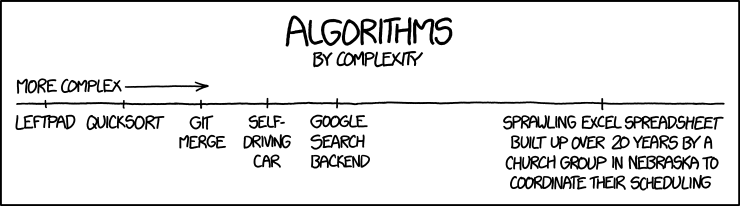
\includegraphics{images/algorithms} \\
    \footnotesize\sffamily%
    Tiré de \href{https://xkcd.com/927/}{XKCD.com}
  \end{minipage}
\end{figure}


\section{Exercices}
\label{sec:algorithmes:exercices}

\Opensolutionfile{solutions}[solutions-algorithmes]

\begin{Filesave}{solutions}
\section*{Chapitre \ref*{chap:algorithmes}}
\addcontentsline{toc}{section}{Chapitre \protect\ref*{chap:algorithmes}}

\begingroup
%% modifications locales au style des listings
% \lstset{%
%   frame=single,
%   numbers=none,
%   basicstyle=\normalfont\ttfamily\NoAutoSpacing}

\end{Filesave}

\begin{exercice}
  Écrire l'algorithme d'une fonction \code{quadroots} qui prend en
  arguments les coefficients (réels) $a$, $b$ et $c$ d'un polynôme du
  second degré $a x^2 + b x + c$ et qui calcule les racines du
  polynôme avec la formule bien connue
  \begin{equation*}
    \frac{-b \pm \sqrt{b^2 - 4ac}}{2a}.
  \end{equation*}
  La fonction doit retourner deux, une ou aucune racine selon que le
  discriminant $b^2 - 4ac$ est positif, nul ou négatif, dans l'ordre.
  \begin{sol}
    Voici des versions en langage naturel et en pseudocode.

    \begin{algorithme}
      Calculer les racines du polynôme $a x^2 + b x + c$ à partir des
      coefficients réels $a$, $b$ et $c$.
      \begin{enumerate}[1.]
      \item Poser $d \leftarrow b^2 - 4ac$.
      \item Si $d < 0$, retourner un résultat vide.
      \item Si $d = 0$, retourner $-b/(2a)$.
      \item Retourner $(-b - \sqrt{d})/(2a)$ et
        $(-b + \sqrt{d})/(2a)$.
      \end{enumerate}
    \end{algorithme}

    \begin{algorithme}
      Calculer les racines du polynôme $a x^2 + b x + c$ à partir des
      coefficients réels $a$, $b$ et $c$.
      \begin{Schunk}
\begin{Verbatim}[commandchars=\\\{\}]
quadroots(réel a, réel b, réel c)
  d \leftarrow b^2 - 4 \times a \times c
  Si (d < 0)
    Retourner NULL
  Si (d = 0)
    Retourner -b/(2 \times a)
  x \leftarrow (-b - sqrt(d))/(2 \times a)
  y \leftarrow (-b + sqrt(d))/(2 \times a)
  Retourner x et y
Fin quadroots
\end{Verbatim}
      \end{Schunk}
    \end{algorithme}
  \end{sol}
\end{exercice}

\begin{exercice}
  Expliquer dans vos mots pourquoi la clause «sinon» n'est jamais
  nécessaire lorsque la \meta{conséquence} d'une instruction
  conditionnelle à deux volets contient une instruction «Retourner».
  \begin{sol}
    Si la \meta{condition} d'une instruction conditionnelle est
    vraie, la fonction se termine avec l'instruction «Retourner».
    Toutes les instructions qui suivent la clause «Si
    \meta{condition}, alors \dots» ne peuvent donc être évaluées que
    lorsque la \meta{condition} est fausse. Inutile de les protéger
    par une clause «sinon».

    Par exemple, supposons qu'une fonction contient les instructions
    suivantes:
    \begin{Schunk}
\begin{Verbatim}[commandchars=\\\{\}]
Si \meta{condition}
  \meta{conséquence}
sinon
  \meta{alternative}
\meta{instruction}
\end{Verbatim}
    \end{Schunk}
    Avec une telle structure, l'\meta{instruction} sera évaluée en
    tout temps, que la \meta{condition} soit vraie ou fausse. Or, si la
    \meta{conséquence} contient «Retourner», tant l'\meta{alternative}
    que l'\meta{instruction} ne seront évaluée que lorsque la
    \meta{condition} est fausse. La formulation ci-dessous est donc
    tout à fait équivalente.
    \begin{Schunk}
\begin{Verbatim}[commandchars=\\\{\}]
Si \meta{condition}
  \meta{conséquence}
\meta{alternative}
\meta{instruction}
\end{Verbatim}
    \end{Schunk}
  \end{sol}
\end{exercice}

\begin{exercice}
  Plusieurs algorithmes comportent une étape d'échange de deux
  valeurs, que l'on pourrait symboliser par $m \leftrightarrow n$.
  \begin{enumerate}
  \item Expliquer comment effectuer l'opération $m \leftrightarrow n$
    sans perdre l'une ou l'autre des valeurs $m$ et $n$.
    \emph{Indice}: il faut avoir recours à une troisième variable
    temporaire, disons $t$.
  \item Expliquer comment réordonner les valeurs $(a, b, c, d)$ en
    $(b, c, d, a)$ en effectuant un minimum de remplacements.
  \end{enumerate}
  \begin{sol}
    \begin{enumerate}
    \item Les étapes à suivre sont, dans l'ordre: $t \leftarrow m$, $m
      \leftarrow n$, $n \leftarrow t$.
    \item Une solution qui ne requiert que cinq remplacements est:
      $t \leftarrow a$, $a \leftarrow b$, $b \leftarrow c$,
      $c \leftarrow d$, $d \leftarrow t$.
    \end{enumerate}
  \end{sol}
\end{exercice}

\begin{exercice}
  Soit $p$ et $q$ des expressions logiques. Compléter les tables de
  vérité ci-dessous.
  \begin{multicols}{2}
    \begin{enumerate}
    \item
      \begin{tabular}{ccc}
        \toprule
        $p$ & $q$ & $p$ ET $q$ \\
        \midrule
        V & V \\
        V & F \\
        F & V \\
        F & F \\
        \bottomrule
      \end{tabular}
      \columnbreak
    \item
      \begin{tabular}{ccc}
        \toprule
        $p$ & $q$ & $p$ OU $q$ \\
        \midrule
        V & V \\
        V & F \\
        F & V \\
        F & F \\
        \bottomrule
      \end{tabular}
    \end{enumerate}
  \end{multicols}
  \begin{sol}
    Nous pouvons compléter les tables de vérité directement à partir
    des définitions des opérateurs ET et OU fournies à la
    \autoref{sec:algorithmes:if-else}:
    \begin{multicols}{2}
      \begin{enumerate}
      \item
        \begin{tabular}{ccc}
          \toprule
          $p$ & $q$ & $p$ ET $q$ \\
          \midrule
          V & V & V \\
          V & F & F \\
          F & V & F \\
          F & F & F \\
          \bottomrule
        \end{tabular}
        \columnbreak
      \item
        \begin{tabular}{ccc}
          \toprule
          $p$ & $q$ & $p$ OU $q$ \\
          \midrule
          V & V & V \\
          V & F & V \\
          F & V & V \\
          F & F & F \\
          \bottomrule
        \end{tabular}
      \end{enumerate}
    \end{multicols}
  \end{sol}
\end{exercice}

\begin{exercice}
  La notation en algèbre booléenne est plus compacte et lisible que
  celle utilisée à la \autoref{sec:algorithmes:if-else}. Si $p$ et $q$
  sont des expressions logiques, on représente généralement $p$ ET $q$
  par $p \wedge q$, $p$ OU $q$ par $p \vee q$, et NON $p$ par
  $\overline{p}$.

  Soit $p$, $q$ et $r$ des expressions logiques. Démontrer à l'aide de
  tables de vérité les identités logiques suivantes.
  \begin{enumerate}
  \item $p \wedge (q \vee r) = (p \wedge q) \vee (p \wedge r)$
  \item $p \vee (q \wedge r) = (p \vee q) \wedge (p \vee r)$
  \item $\overline{p \wedge q} = \overline{p} \vee \overline{q}$
  \item $\overline{p \vee q} = \overline{p} \wedge \overline{q}$
  \item $(p \wedge q) \vee (\overline{p} \wedge r) = (p \wedge q) \vee (\overline{p} \wedge
    r) \vee (q \wedge r)$
  \end{enumerate}
  \begin{sol}
    Tel que proposé dans l'énoncé, tous les résultats se démontrent à
    l'aide de tables de vérité.
    \begin{enumerate}
    \item
      \begin{tabularx}{\linewidth}{*{7}{c}>{\centering\arraybackslash}X}
        \toprule
        $p$ & $q$ & $r$ & $p \wedge q$ & $p \wedge r$ & $q \vee r$ & $p \wedge (q \vee r)$ & $(p \wedge q) \newline\vee (p \wedge r)$
        \\
        \midrule
        V & V & V & V & V & V & V & V \\
        V & V & F & V & F & V & V & V \\
        V & F & V & F & V & V & V & V \\
        V & F & F & F & F & F & F & F \\
        F & V & V & F & F & V & F & F \\
        F & V & F & F & F & V & F & F \\
        F & F & V & F & F & V & F & F \\
        F & F & F & F & F & F & F & F \\
        \bottomrule
      \end{tabularx}
    \item
      \begin{tabularx}{\linewidth}{*{7}{c}>{\centering\arraybackslash}X}
        \toprule
        $p$ & $q$ & $r$ & $p \vee q$ & $p \vee r$ & $q \wedge r$ & $p \vee (q \wedge r)$ & $(p \vee q) \newline\wedge (p \vee r)$
        \\
        \midrule
        V & V & V & V & V & V & V & V \\
        V & V & F & V & V & F & V & V \\
        V & F & V & V & V & F & V & V \\
        V & F & F & V & V & F & V & V \\
        F & V & V & V & V & V & V & V \\
        F & V & F & V & F & F & F & F \\
        F & F & V & F & V & F & F & F \\
        F & F & F & F & F & F & F & F \\
        \bottomrule
      \end{tabularx}
    \item
      \begin{tabular}{*{6}{c}}
        \toprule
        $p$ & $q$ & $\overline{p}$ & $\overline{q}$ & $\overline{p \wedge q}$ & $\overline{p} \vee \overline{q}$ \\
        \midrule
        V & V & F & F & F & F \\
        V & F & F & V & V & V \\
        F & V & V & F & V & V \\
        F & F & V & V & V & V \\
        \bottomrule
      \end{tabular}
    \item
      \begin{tabular}{*{6}{c}}
        \toprule
        $p$ & $q$ & $\overline{p}$ & $\overline{q}$ & $\overline{p \vee q}$ & $\overline{p} \wedge \overline{q}$ \\
        \midrule
        V & V & F & F & F & F \\
        V & F & F & V & F & F \\
        F & V & V & F & F & F \\
        F & F & V & V & V & V \\
        \bottomrule
      \end{tabular}
    \item
      \begin{tabularx}{\linewidth}{*{6}{c}>{\centering\arraybackslash}X>{\centering\arraybackslash}X}
        \toprule
        $p$ & $q$ & $r$ & $p \wedge q$ & $\overline{p} \wedge r$ & $q \wedge r$ & $(p \wedge q) \newline\vee (\overline{p} \wedge r)$ & $(p \wedge q) \newline\vee (\overline{p} \wedge r) \newline\vee (q \wedge r)$
        \\
        \midrule
        V & V & V & V & F & V & V & V \\
        V & V & F & V & F & F & V & V \\
        V & F & V & F & F & F & F & F \\
        V & F & F & F & F & F & F & F \\
        F & V & V & F & V & V & V & V \\
        F & V & F & F & F & F & F & F \\
        F & F & V & F & V & F & V & V \\
        F & F & F & F & F & F & F & F \\
        \bottomrule
      \end{tabularx}
    \end{enumerate}
  \end{sol}
\end{exercice}

\begin{exercice}
  Écrire une version récursive présentée en pseudocode de l'algorithme
  d'\index{Euclide@Euclide (algorithme)}Euclide.
  \begin{sol}
    Tel que mentionné à la \autoref{sec:algorithmes:iteration}, les
    algorithmes récusifs s'expriment généralement mieux en pseudocode.
    L'algorithme d'\index{Euclide@Euclide (algorithme)}Euclide est
    particulièrement simple exprimé ainsi.
    \begin{Schunk}
\begin{Verbatim}
PGCD(entier m, entier n)
  Si (n = 0) retourner m
  Retourner PGCD(n, m mod n)
Fin PGCD
\end{Verbatim}
    \end{Schunk}
  \end{sol}
\end{exercice}

\begin{exercice}
  La suite de \index{Fibonacci}Fibonacci est une suite de
  nombres entiers très connue. Les deux premiers termes de la suite
  sont $0$ et $1$ et tous les autres sont la somme des deux termes
  précédents. Mathématiquement, les valeurs de la suite de Fibonacci
  sont données par la fonction
  \begin{align*}
    f(0) &= 0 \\
    f(1) &= 1 \\
    f(n) & = f(n - 1) + f(n - 2), \quad n \geq 2.
  \end{align*}
  Le quotient de deux termes successifs converge vers
  $\phi = (1 + \sqrt{5})/2$, le nombre d'or.\footnote{%
    On prête au nombre d'or toutes sortes de propriétés, certaines
    même d'ordre mystique. Il est en tout cas au cœur d'un des romans
    les plus vendus de tous les temps, \emph{Da~Vinci Code} (Dan
    Brown, 2003).} %
  Le calcul de $f(n)$ se prête tout naturellement à une mise en œuvre
  récursive.
  \begin{enumerate}
  \item Proposer un algorithme récursif pour calculer la valeur $f(n)$
    de la suite de Fibonacci.
  \item Calculer les 10 premiers nombres de Fibonacci.
  \item L'algorithme récursif direct de la suite de Fibonacci est
    terriblement inefficace puisqu'il répète plusieurs calculs un
    grand nombre de fois. Pour vous en convaincre, écrivez au long
    tous les calculs requis par l'algorithme pour calculer $f(5)$.
  \item Proposer un algorithme itératif en langage naturel pour
    calculer les nombres de Fibonacci.
  \end{enumerate}
  \begin{sol}
    \begin{enumerate}
    \item L'algorithme ci-dessous permet de calculer les nombres de
      Fibonacci de manière récursive.
      \begin{algorithme}[Suite de Fibonacci]
        \label{algo:algorithmes:Fibonacci}
        Calculer la valeur $f(n)$ de la suite de
        \index{Fibonacci}Fibonacci pour un entier non négatif $n$.
        \begin{Schunk}
\begin{Verbatim}
Fib(entier n)
  Si (n = 0), retourner 0
  Si (n = 1), retourner 1
  Retourner Fib(n - 2) + Fib(n - 1)
Fin Fib
\end{Verbatim}
        \end{Schunk}
      \end{algorithme}
    \item Les 10 premiers nombres de Fibonacci sont:
      $0, 1, 1, 2, 3, 5, 8, 13, 21, 34$.
    \item En décomposant la méthode de calcul des nombres de Fibonacci
      employée par l'\autoref{algo:algorithmes:Fibonacci}, on obtient:
      \begin{align*}
        f(5)
        &= f(4) + f(3) \\
        &= (f(3) + f(2)) + (f(2) + f(1)) \displaybreak[0]\\
        &= ((f(2) + f(1)) + (f(1) + f(0))) \\
        &\phantom{=} + ((f(1) + f(0)) + f(1)) \displaybreak[0]\\
        &= (((f(1) + f(0)) + f(1)) + (f(1) + f(0))) \\
        &\phantom{=} + ((f(1) + f(0)) + f(1)).
      \end{align*}
      Plusieurs calculs sont redondants. Il faut calculer $f(1)$ pas
      moins de cinq fois et le calcul de $f(3)$ dès la première
      égalité ci-dessus n'est qu'une reprise d'un calcul effectué par
      ailleurs. En fait, cet algorithme est souvent utilisé comme cas
      pathologique dans les ouvrages d'algorithmique.
    \item L'algorithme ci-dessous permet de calculer les nombres de
      Fibonacci de manière itérative.
      \begin{algorithme}[Suite de Fibonacci]
        \label{algo:algorithmes:Fibonacci-iter}
        Calculer la valeur $f(n)$ de la suite de
        \index{Fibonacci}Fibonacci pour un entier non négatif $n$.
        \begin{enumerate}[1.]
        \item Poser $a \leftarrow 0$, $b \leftarrow 1$ et
          $i \leftarrow 2$.
        \item Si $n = 0$, retourner $a$.
        \item Si $n = 1$, retourner $b$.
        \item Poser $r \leftarrow a + b$.
        \item Si $i = n$, retourner la valeur $r$.
        \item Poser $a \leftarrow b$ et $b \leftarrow r$,
        \item Incrémenter le compteur $i$: $i \leftarrow i + 1$, puis
          retouner à l'étape 4.
        \end{enumerate}
      \end{algorithme}
    \end{enumerate}
  \end{sol}
\end{exercice}

\begin{exercice}
  L'algorithme suivant permet de calculer la valeur de la fonction de
  \index{Ackermann (fonction)}Ackermann $A(x, y)$ pour des entiers non
  négatifs $x$ et $y$ telle que définie dans
  \citet{Sussman:scheme:1996}.

  \begin{Schunk}
\begin{Verbatim}[commandchars=\\\{\}]
A(entier x, entier y)
  Si (y = 0)
    Retourner 0
  Sinon Si (x = 0)
    Retourner 2 \times y
  Sinon Si (y = 1)
    Retourner 2
  Sinon
    Retourner A(x - 1, A(x, y - 1))
Fin A
\end{Verbatim}
  \end{Schunk}

  Calculer la valeur de $A(1, 10)$.
  \begin{sol}
    On a
    \begin{align*}
      A(1, 10)
      &= A(0, A(1, 9)) \\
      &= A(0, A(0, A(1, 8))) \\
      &= A(0, A(0, A(0, A(1, 7)))) \\
      &= A(0, A(0, A(0, A(0, A(1, 6))))) \displaybreak[0] \\
      &= A(0, A(0, A(0, A(0, A(0, A(1, 5)))))) \\
      &= A(0, A(0, A(0, A(0, A(0, A(0, A(1, 4))))))) \\
      &= A(0, A(0, A(0, A(0, A(0, A(0, A(0, A(1, 3)))))))) \\
      &= A(0, A(0, A(0, A(0, A(0, A(0, A(0, A(0, A(1, 2))))))))) \displaybreak[0] \\
      &= A(0, A(0, A(0, A(0, A(0, A(0, A(0, A(0, A(0, A(1, 1)))))))))) \\
      &= A(0, A(0, A(0, A(0, A(0, A(0, A(0, A(0, A(0, 2))))))))) \\
      &= A(0, A(0, A(0, A(0, A(0, A(0, A(0, A(0, 4)))))))) \\
      &= A(0, A(0, A(0, A(0, A(0, A(0, A(0, 8))))))) \displaybreak[0] \\
      &= A(0, A(0, A(0, A(0, A(0, A(0, 16)))))) \\
      &= A(0, A(0, A(0, A(0, A(0, 32))))) \\
      &= A(0, A(0, A(0, A(0, 64)))) \\
      &= A(0, A(0, A(0, 128))) \displaybreak[0] \\
      &= A(0, A(0, 256)) \\
      &= A(0, 512) \\
      &= \nombre{1024}.
    \end{align*}
  \end{sol}
\end{exercice}

\begin{exercice}
  Soit un algorithme avec $n$ entrées qui génère des valeurs pour
  chacun des carrés unitaires à la surface d'un cube
  $n \times n \times n$. Calculer la performance de l'algorithme. %
  \citep[Tiré de][]{Stephens:algorithms:2013}
  \begin{sol}
    Si le cube a $n$ unités de côté, sa surface est $6 n^2$. La
    performance de l'algorithme est donc $O(n^2)$. Nous pouvons
    obtenir cette réponse simplement en remarquant que l'algorithme
    doit calculer une aire.
  \end{sol}
\end{exercice}

\begin{exercice}
  Soit un algorithme avec $n$ entrées qui génère des valeurs pour
  chacun des cubes unitaires sur le pourtour d'un cube
  $n \times n \times n$, tel qu'illustré à la
  \autoref{fig:algorithmes:cubes-pourtour}. Calculer la performance de
  l'algorithme. %
  \citep[Tiré de][]{Stephens:algorithms:2013}
  \begin{sol}
    Le cube $n \times n \times n$ compte $8$ coins et $12$ côtés. La
    longueur de chaque côté en excluant les extrémités est $n - 2$. Le
    nombre total de cubes sur le pourtour est donc
    $12(n - 2) + 8 = 12n - 16$. La performance de l'algorithme est
    donc $O(n)$. Nous pouvons aussi obtenir cette réponse en
    remarquant que l'algorithme doit en définitive calculer une
    longueur.
  \end{sol}

  \begin{figure}
    \centering
    \setlength{\unitlength}{5mm}
    \thicklines
    %% unités de base en blanc
\savebox{\cube}(1.5,1.3)[bl]{%
  \roundjoin
  \color{white}
  \polygon*(0,0)(0,1)(1,1)(1,0)
  \color{lightgray}
  \polygon*(0,1)(0.5,1.3)(1.5,1.3)(1,1)
  \color{gray}
  \polygon*(1,1)(1.5,1.3)(1.5,0.3)(1,0)
  \color{black}
  \moveto(0,0)
  \lineto(0,1) \lineto(1,1) \lineto(1,0)
  \closepath
  \strokepath
  \polyline(0,1)(0.5,1.3)(1.5,1.3)(1,1)(0,1)
  \polyline(1,1)(1.5,1.3)(1.5,0.3)(1,0)(1,1)
}
\savebox{\mcube}(1,1.5)[bl]{%
  \roundjoin
  \color{lightgray}
  \polygon*(0,0)(0,1)(1,1)(1,0)
  \color{gray}
  \polygon*(0,1)(0.5,1.3)(1.5,1.3)(1,1)
  \color{darkgray}
  \polygon*(1,1)(1.5,1.3)(1.5,0.3)(1,0)
  \color{black}
  \moveto(0,0)
  \lineto(0,1) \lineto(1,1) \lineto(1,0)
  \closepath
  \strokepath
  \polyline(0,1)(0.5,1.3)(1.5,1.3)(1,1)(0,1)
  \polyline(1,1)(1.5,1.3)(1.5,0.3)(1,0)(1,1)
}
\savebox{\dcube}(1,1.5)[bl]{%
  \roundjoin
  \color{gray}
  \polygon*(0,0)(0,1)(1,1)(1,0)
  \color{darkgray}
  \polygon*(0,1)(0.5,1.3)(1.5,1.3)(1,1)
  \color{black!85}
  \polygon*(1,1)(1.5,1.3)(1.5,0.3)(1,0)
  \color{black}
  \moveto(0,0)
  \lineto(0,1) \lineto(1,1) \lineto(1,0)
  \closepath
  \strokepath
  \polyline(0,1)(0.5,1.3)(1.5,1.3)(1,1)(0,1)
  \polyline(1,1)(1.5,1.3)(1.5,0.3)(1,0)(1,1)
}
\savebox{\ligne}(0,0)[bl]{%
  \multiput(0.0,0.0)(1,0){5}{\usebox{\cube}}
}
\savebox{\colonne}(0,0)[bl]{%
  \multiput(0.0,0.0)(0,1){3}{\usebox{\cube}}
}
\savebox{\carotte}(0,0)[bl]{%
  \multiput(1.5,0.9)(-0.5,-0.3){4}{\usebox{\cube}}
}
\savebox{\matrice}(0,0)[bl]{%
  \multiput(0.0,0.0)(0,1){3}{\usebox{\ligne}}
}
\savebox{\trancheh}(0,0)[bl]{%
  \multiput(1.5,0.9)(-0.5,-0.3){4}{\usebox{\ligne}}
}
\savebox{\tranchev}(0,0)[bl]{%
  \multiput(1.5,0.9)(-0.5,-0.3){4}{\usebox{\colonne}}
}
\savebox{\tableau}(0,0)[bl]{
  \multiput(1.5,0.9)(-0.5,-0.3){4}{\usebox{\matrice}}
}
\savebox{\cubedouble}(3,2.6)[bl]{%
  \roundjoin
  \color{white}
  \polygon*(0,0)(0,2)(2,2)(2,0)
  \color{lightgray}
  \polygon*(0,2)(1,2.6)(3,2.6)(2,2)
  \color{gray}
  \polygon*(2,2)(3,2.6)(3,0.6)(2,0)
  \color{black}
  \moveto(0,0)
  \lineto(0,2) \lineto(2,2) \lineto(2,0)
  \closepath
  \strokepath
  \polyline(0,2)(1,2.6)(3,2.6)(2,2)(0,2)
  \polyline(2,2)(3,2.6)(3,0.6)(2,0)(2,2)
}
\savebox{\polygone}(6,2.6)[bl]{%
  \roundjoin
  \color{white}
  \polygon*(0,0)(0,2)(5,2)(5,0)
  \color{lightgray}
  \polygon*(0,2)(1.0,2.6)(6,2.6)(5,2)
  \color{gray}
  \polygon*(5,2)(6,2.6)(6,0.6)(5,0)
  \color{black}
  \moveto(0,0)
  \lineto(0,2) \lineto(5,2) \lineto(5,0)
  \closepath
  \strokepath
  \polyline(0,2)(1.0,2.6)(6,2.6)(5,2)(0,2)
  \polyline(5,2)(6,2.6)(6,0.6)(5,0)(5,2)
}
\savebox{\gpolygone}(14.25,4.55)[bl]{%
  \roundjoin
  \color{white}
  \polygon*(0,0)(0,3.5)(12.5,3.5)(12.5,0)
  \color{lightgray}
  \polygon*(0,3.5)(1.75,4.55)(14.25,4.55)(12.5,3.5)
  \color{gray}
  \polygon*(12.5,3.5)(14.25,4.55)(14.25,1.05)(12.5,0)
  \color{black}
  \moveto(0,0)
  \lineto(0,3.5) \lineto(12.5,3.5) \lineto(12.5,0)
  \closepath
  \strokepath
  \polyline(0,3.5)(1.75,4.55)(14.25,4.55)(12.5,3.5)(0,3.5)
  \polyline(12.5,3.5)(14.25,4.55)(14.25,1.05)(12.5,0)(12.5,3.5)
}

%% versions colorées
\savebox{\ccube}(1,1.5)[bl]{%
  \roundjoin
  \color{indexedface}
  \polygon*(0,0)(0,1)(1,1)(1,0)
  \color{indexedtop}
  \polygon*(0,1)(0.5,1.3)(1.5,1.3)(1,1)
  \color{indexedside}
  \polygon*(1,1)(1.5,1.3)(1.5,0.3)(1,0)
  \color{black}
  \moveto(0,0)
  \lineto(0,1) \lineto(1,1) \lineto(1,0)
  \closepath
  \strokepath
  \polyline(0,1)(0.5,1.3)(1.5,1.3)(1,1)(0,1)
  \polyline(1,1)(1.5,1.3)(1.5,0.3)(1,0)(1,1)
}
\savebox{\mccube}(1,1.5)[bl]{%
  \roundjoin
  \color{mindexedface}
  \polygon*(0,0)(0,1)(1,1)(1,0)
  \color{mindexedtop}
  \polygon*(0,1)(0.5,1.3)(1.5,1.3)(1,1)
  \color{mindexedside}
  \polygon*(1,1)(1.5,1.3)(1.5,0.3)(1,0)
  \color{black}
  \moveto(0,0)
  \lineto(0,1) \lineto(1,1) \lineto(1,0)
  \closepath
  \strokepath
  \polyline(0,1)(0.5,1.3)(1.5,1.3)(1,1)(0,1)
  \polyline(1,1)(1.5,1.3)(1.5,0.3)(1,0)(1,1)
}
\savebox{\dccube}(1,1.5)[bl]{%
  \roundjoin
  \color{dindexedface}
  \polygon*(0,0)(0,1)(1,1)(1,0)
  \color{dindexedtop}
  \polygon*(0,1)(0.5,1.3)(1.5,1.3)(1,1)
  \color{dindexedside}
  \polygon*(1,1)(1.5,1.3)(1.5,0.3)(1,0)
  \color{black}
  \moveto(0,0)
  \lineto(0,1) \lineto(1,1) \lineto(1,0)
  \closepath
  \strokepath
  \polyline(0,1)(0.5,1.3)(1.5,1.3)(1,1)(0,1)
  \polyline(1,1)(1.5,1.3)(1.5,0.3)(1,0)(1,1)
}
\savebox{\cligne}(0,0)[bl]{%
  \multiput(0.0,0.0)(1,0){5}{\usebox{\ccube}}
}
\savebox{\ccolonne}(0,0)[bl]{%
  \multiput(0.0,0.0)(0,1){3}{\usebox{\ccube}}
}
\savebox{\ccarotte}(0,0)[bl]{%
  \multiput(1.5,0.9)(-0.5,-0.3){4}{\usebox{\ccube}}
}
\savebox{\cmatrice}(0,0)[bl]{%
  \multiput(0.0,0.0)(0,1){3}{\usebox{\cligne}}
}
\savebox{\ctrancheh}(0,0)[bl]{%
  \multiput(1.5,0.9)(-0.5,-0.3){4}{\usebox{\cligne}}
}
\savebox{\ctranchev}(0,0)[bl]{%
  \multiput(1.5,0.9)(-0.5,-0.3){4}{\usebox{\ccolonne}}
}
\savebox{\ctableau}(0,0)[bl]{
  \multiput(1.5,0.9)(-0.5,-0.3){4}{\usebox{\cmatrice}}
}

    \begin{picture}(11,3.9)(-4.5,0)
      \multiput(1.0,0.6)(1,0){3}{\usebox{\cube}}
      \multiput(0.5,0.3)(2,0){2}{\usebox{\cube}}
      \multiput(0.0,0.0)(1,0){3}{\usebox{\cube}}

      \multiput(1.0,1.6)(2,0){2}{\usebox{\cube}}
      \multiput(0.0,1.0)(2,0){2}{\usebox{\cube}}

      \multiput(1.0,2.6)(1,0){3}{\usebox{\cube}}
      \multiput(0.5,2.3)(2,0){2}{\usebox{\cube}}
      \multiput(0.0,2.0)(1,0){3}{\usebox{\cube}}

      \put(-4.5,1.5){\makebox(0,0)[l]{$n = 3$}}
    \end{picture} \\
    \bigskip
    \begin{picture}(11,5.2)(-4,0)
      \multiput(1.5,0.9)(1,0){4}{\usebox{\cube}}
      \multiput(1.0,0.6)(3,0){2}{\usebox{\cube}}
      \multiput(0.5,0.3)(3,0){2}{\usebox{\cube}}
      \multiput(0.0,0.0)(1,0){4}{\usebox{\cube}}

      \multiput(1.5,1.9)(3,0){2}{\usebox{\cube}}
      \multiput(0.0,1.0)(3,0){2}{\usebox{\cube}}

      \multiput(1.5,2.9)(3,0){2}{\usebox{\cube}}
      \multiput(0.0,2.0)(3,0){2}{\usebox{\cube}}

      \multiput(1.5,3.9)(1,0){4}{\usebox{\cube}}
      \multiput(1.0,3.6)(3,0){2}{\usebox{\cube}}
      \multiput(0.5,3.3)(3,0){2}{\usebox{\cube}}
      \multiput(0.0,3.0)(1,0){4}{\usebox{\cube}}

      \put(-4,2){\makebox(0,0)[l]{$n = 4$}}
    \end{picture} \\
    \bigskip
    \begin{picture}(11,6.5)(-3.5,0)
      \multiput(2.0,1.2)(1,0){5}{\usebox{\cube}}
      \multiput(1.5,0.9)(4,0){2}{\usebox{\cube}}
      \multiput(1.0,0.6)(4,0){2}{\usebox{\cube}}
      \multiput(0.5,0.3)(4,0){2}{\usebox{\cube}}
      \multiput(0.0,0.0)(1,0){5}{\usebox{\cube}}

      \multiput(2.0,2.2)(4,0){2}{\usebox{\cube}}
      \multiput(0.0,1.0)(4,0){2}{\usebox{\cube}}

      \multiput(2.0,3.2)(4,0){2}{\usebox{\cube}}
      \multiput(0.0,2.0)(4,0){2}{\usebox{\cube}}

      \multiput(2.0,4.2)(4,0){2}{\usebox{\cube}}
      \multiput(0.0,3.0)(4,0){2}{\usebox{\cube}}

      \multiput(2.0,5.2)(1,0){5}{\usebox{\cube}}
      \multiput(1.5,4.9)(4,0){2}{\usebox{\cube}}
      \multiput(1.0,4.6)(4,0){2}{\usebox{\cube}}
      \multiput(0.5,4.3)(4,0){2}{\usebox{\cube}}
      \multiput(0.0,4.0)(1,0){5}{\usebox{\cube}}

      \put(-3.5,2.5){\makebox(0,0)[l]{$n = 5$}}
    \end{picture}
    \caption{Illustrations pour un algorithme qui génère des valeurs
      sur le pourtour d'un cube}
    \label{fig:algorithmes:cubes-pourtour}
  \end{figure}
\end{exercice}

\begin{exercice}
  Soit un algorithme avec $n$ entrées qui génère des valeurs pour
  chacun des carrés unitaires d'une pyramide comme dans le jeu
  classique \link{https://fr.wikipedia.org/wiki/Q*bert}{Q*bert}, tel
  qu'illustré à la \autoref{fig:algorithmes:q*bert}. Supposer que les
  cubes invisibles sont présents de telle sorte que les structures
  sont pleines. Calculer la performance de l'algorithme. %
  \citep[Tiré de][]{Stephens:algorithms:2013}
  \begin{sol}
    L'étage $k$ d'une pyramide de $n$ étage compte $k(k + 1)/2$ cubes.
    Le nombre total de cubes est donc égal à
    \begin{equation*}
      \sum_{k = 1}^n \frac{k (k + 1)}{2}.
    \end{equation*}
    À l'aide des identités
    \begin{align*}
      \sum_{k = 1}^n k &= \frac{n (n + 1)}{2} \\
      \sum_{k = 1}^n k^2 &= \frac{n (n + 1) (2n + 1)}{6},
    \end{align*}
    on obtient avec un peu d'algèbre que
    \begin{equation*}
      \sum_{k = 1}^n \frac{k (k + 1)}{2} = \frac{n^3 + 3 n^2 + 2n}{6}.
    \end{equation*}
    La performance de l'algorithme est donc $O(n^3)$, une réponse
    intuitivement claire dans la mesure où l'algorithme calcule un
    volume.
  \end{sol}

  \begin{figure}
    \centering
    \setlength{\unitlength}{8mm}
    \thicklines
    %% unités de base en blanc
\savebox{\cube}(1.5,1.3)[bl]{%
  \roundjoin
  \color{white}
  \polygon*(0,0)(0,1)(1,1)(1,0)
  \color{lightgray}
  \polygon*(0,1)(0.5,1.3)(1.5,1.3)(1,1)
  \color{gray}
  \polygon*(1,1)(1.5,1.3)(1.5,0.3)(1,0)
  \color{black}
  \moveto(0,0)
  \lineto(0,1) \lineto(1,1) \lineto(1,0)
  \closepath
  \strokepath
  \polyline(0,1)(0.5,1.3)(1.5,1.3)(1,1)(0,1)
  \polyline(1,1)(1.5,1.3)(1.5,0.3)(1,0)(1,1)
}
\savebox{\mcube}(1,1.5)[bl]{%
  \roundjoin
  \color{lightgray}
  \polygon*(0,0)(0,1)(1,1)(1,0)
  \color{gray}
  \polygon*(0,1)(0.5,1.3)(1.5,1.3)(1,1)
  \color{darkgray}
  \polygon*(1,1)(1.5,1.3)(1.5,0.3)(1,0)
  \color{black}
  \moveto(0,0)
  \lineto(0,1) \lineto(1,1) \lineto(1,0)
  \closepath
  \strokepath
  \polyline(0,1)(0.5,1.3)(1.5,1.3)(1,1)(0,1)
  \polyline(1,1)(1.5,1.3)(1.5,0.3)(1,0)(1,1)
}
\savebox{\dcube}(1,1.5)[bl]{%
  \roundjoin
  \color{gray}
  \polygon*(0,0)(0,1)(1,1)(1,0)
  \color{darkgray}
  \polygon*(0,1)(0.5,1.3)(1.5,1.3)(1,1)
  \color{black!85}
  \polygon*(1,1)(1.5,1.3)(1.5,0.3)(1,0)
  \color{black}
  \moveto(0,0)
  \lineto(0,1) \lineto(1,1) \lineto(1,0)
  \closepath
  \strokepath
  \polyline(0,1)(0.5,1.3)(1.5,1.3)(1,1)(0,1)
  \polyline(1,1)(1.5,1.3)(1.5,0.3)(1,0)(1,1)
}
\savebox{\ligne}(0,0)[bl]{%
  \multiput(0.0,0.0)(1,0){5}{\usebox{\cube}}
}
\savebox{\colonne}(0,0)[bl]{%
  \multiput(0.0,0.0)(0,1){3}{\usebox{\cube}}
}
\savebox{\carotte}(0,0)[bl]{%
  \multiput(1.5,0.9)(-0.5,-0.3){4}{\usebox{\cube}}
}
\savebox{\matrice}(0,0)[bl]{%
  \multiput(0.0,0.0)(0,1){3}{\usebox{\ligne}}
}
\savebox{\trancheh}(0,0)[bl]{%
  \multiput(1.5,0.9)(-0.5,-0.3){4}{\usebox{\ligne}}
}
\savebox{\tranchev}(0,0)[bl]{%
  \multiput(1.5,0.9)(-0.5,-0.3){4}{\usebox{\colonne}}
}
\savebox{\tableau}(0,0)[bl]{
  \multiput(1.5,0.9)(-0.5,-0.3){4}{\usebox{\matrice}}
}
\savebox{\cubedouble}(3,2.6)[bl]{%
  \roundjoin
  \color{white}
  \polygon*(0,0)(0,2)(2,2)(2,0)
  \color{lightgray}
  \polygon*(0,2)(1,2.6)(3,2.6)(2,2)
  \color{gray}
  \polygon*(2,2)(3,2.6)(3,0.6)(2,0)
  \color{black}
  \moveto(0,0)
  \lineto(0,2) \lineto(2,2) \lineto(2,0)
  \closepath
  \strokepath
  \polyline(0,2)(1,2.6)(3,2.6)(2,2)(0,2)
  \polyline(2,2)(3,2.6)(3,0.6)(2,0)(2,2)
}
\savebox{\polygone}(6,2.6)[bl]{%
  \roundjoin
  \color{white}
  \polygon*(0,0)(0,2)(5,2)(5,0)
  \color{lightgray}
  \polygon*(0,2)(1.0,2.6)(6,2.6)(5,2)
  \color{gray}
  \polygon*(5,2)(6,2.6)(6,0.6)(5,0)
  \color{black}
  \moveto(0,0)
  \lineto(0,2) \lineto(5,2) \lineto(5,0)
  \closepath
  \strokepath
  \polyline(0,2)(1.0,2.6)(6,2.6)(5,2)(0,2)
  \polyline(5,2)(6,2.6)(6,0.6)(5,0)(5,2)
}
\savebox{\gpolygone}(14.25,4.55)[bl]{%
  \roundjoin
  \color{white}
  \polygon*(0,0)(0,3.5)(12.5,3.5)(12.5,0)
  \color{lightgray}
  \polygon*(0,3.5)(1.75,4.55)(14.25,4.55)(12.5,3.5)
  \color{gray}
  \polygon*(12.5,3.5)(14.25,4.55)(14.25,1.05)(12.5,0)
  \color{black}
  \moveto(0,0)
  \lineto(0,3.5) \lineto(12.5,3.5) \lineto(12.5,0)
  \closepath
  \strokepath
  \polyline(0,3.5)(1.75,4.55)(14.25,4.55)(12.5,3.5)(0,3.5)
  \polyline(12.5,3.5)(14.25,4.55)(14.25,1.05)(12.5,0)(12.5,3.5)
}

%% versions colorées
\savebox{\ccube}(1,1.5)[bl]{%
  \roundjoin
  \color{indexedface}
  \polygon*(0,0)(0,1)(1,1)(1,0)
  \color{indexedtop}
  \polygon*(0,1)(0.5,1.3)(1.5,1.3)(1,1)
  \color{indexedside}
  \polygon*(1,1)(1.5,1.3)(1.5,0.3)(1,0)
  \color{black}
  \moveto(0,0)
  \lineto(0,1) \lineto(1,1) \lineto(1,0)
  \closepath
  \strokepath
  \polyline(0,1)(0.5,1.3)(1.5,1.3)(1,1)(0,1)
  \polyline(1,1)(1.5,1.3)(1.5,0.3)(1,0)(1,1)
}
\savebox{\mccube}(1,1.5)[bl]{%
  \roundjoin
  \color{mindexedface}
  \polygon*(0,0)(0,1)(1,1)(1,0)
  \color{mindexedtop}
  \polygon*(0,1)(0.5,1.3)(1.5,1.3)(1,1)
  \color{mindexedside}
  \polygon*(1,1)(1.5,1.3)(1.5,0.3)(1,0)
  \color{black}
  \moveto(0,0)
  \lineto(0,1) \lineto(1,1) \lineto(1,0)
  \closepath
  \strokepath
  \polyline(0,1)(0.5,1.3)(1.5,1.3)(1,1)(0,1)
  \polyline(1,1)(1.5,1.3)(1.5,0.3)(1,0)(1,1)
}
\savebox{\dccube}(1,1.5)[bl]{%
  \roundjoin
  \color{dindexedface}
  \polygon*(0,0)(0,1)(1,1)(1,0)
  \color{dindexedtop}
  \polygon*(0,1)(0.5,1.3)(1.5,1.3)(1,1)
  \color{dindexedside}
  \polygon*(1,1)(1.5,1.3)(1.5,0.3)(1,0)
  \color{black}
  \moveto(0,0)
  \lineto(0,1) \lineto(1,1) \lineto(1,0)
  \closepath
  \strokepath
  \polyline(0,1)(0.5,1.3)(1.5,1.3)(1,1)(0,1)
  \polyline(1,1)(1.5,1.3)(1.5,0.3)(1,0)(1,1)
}
\savebox{\cligne}(0,0)[bl]{%
  \multiput(0.0,0.0)(1,0){5}{\usebox{\ccube}}
}
\savebox{\ccolonne}(0,0)[bl]{%
  \multiput(0.0,0.0)(0,1){3}{\usebox{\ccube}}
}
\savebox{\ccarotte}(0,0)[bl]{%
  \multiput(1.5,0.9)(-0.5,-0.3){4}{\usebox{\ccube}}
}
\savebox{\cmatrice}(0,0)[bl]{%
  \multiput(0.0,0.0)(0,1){3}{\usebox{\cligne}}
}
\savebox{\ctrancheh}(0,0)[bl]{%
  \multiput(1.5,0.9)(-0.5,-0.3){4}{\usebox{\cligne}}
}
\savebox{\ctranchev}(0,0)[bl]{%
  \multiput(1.5,0.9)(-0.5,-0.3){4}{\usebox{\ccolonne}}
}
\savebox{\ctableau}(0,0)[bl]{
  \multiput(1.5,0.9)(-0.5,-0.3){4}{\usebox{\cmatrice}}
}

    \begin{minipage}{0.48\linewidth}
      \begin{picture}(7,1.3)(-3,0)
        \put(0.0,0.0){\usebox{\cube}}

        \put(-3.0,0.5){\makebox(0,0)[l]{$n = 1$}}
      \end{picture}
    \end{minipage}
    \hfill
    \begin{minipage}{0.48\linewidth}
      \begin{picture}(7,2.6)(-2,0)
        \multiput(0.0,0.0)(1.5,0.3){2}{\usebox{\cube}}
        \multiput(0.5,1.3)(1.5,0.3){1}{\usebox{\cube}}

        \put(-2.0,1.3){\makebox(0,0)[l]{$n = 2$}}
      \end{picture}
    \end{minipage} \\
    \bigskip
    \begin{minipage}{0.48\linewidth}
      \begin{picture}(7,3.9)(-2,0)
        \multiput(0.0,0.0)(1.5,0.3){3}{\usebox{\cube}}
        \multiput(0.5,1.3)(1.5,0.3){2}{\usebox{\cube}}
        \multiput(1.0,2.6)(1.5,0.3){1}{\usebox{\cube}}

        \put(-2.0,1.8){\makebox(0,0)[l]{$n = 3$}}
      \end{picture}
    \end{minipage}
    \hfill
    \begin{minipage}{0.48\linewidth}
      \begin{picture}(7,5.2)(-1,0)
        \multiput(0.0,0.0)(1.5,0.3){4}{\usebox{\cube}}
        \multiput(0.5,1.3)(1.5,0.3){3}{\usebox{\cube}}
        \multiput(1.0,2.6)(1.5,0.3){2}{\usebox{\cube}}
        \multiput(1.5,3.9)(1.5,0.3){1}{\usebox{\cube}}

        \put(-1.0,2.6){\makebox(0,0)[l]{$n = 4$}}
      \end{picture}
    \end{minipage}
    \caption{Illustrations pour un algorithme qui génère des valeurs
      pour une pyramide comme dans le jeu Q*bert}
    \label{fig:algorithmes:q*bert}
  \end{figure}
\end{exercice}

\begin{exercice}
  Comparer à l'aide d'un graphique pour $n \in (0, 20)$ le rythme de
  croissance des fonctions $\log n$, $\sqrt{n}$, $n$, $n \log n$,
  $n^2$ et $n!$.
  \begin{sol}
    Vous pouvez tracer un graphique regroupant toutes les fonctions
    dans R avec les expressions suivantes.
    \begin{Schunk}
\begin{Sinput}
> plot(0:20, 0:20, type = "n")
> curve(log(x), add = TRUE, col = 1)
> curve(sqrt(x), add = TRUE, col = 2)
> curve(I(x), add = TRUE, col = 3)
> curve(x * log(x), add = TRUE, col = 4)
> curve(x^2, add = TRUE, col = 5)
> curve(factorial(x), add = TRUE, col = 6)
\end{Sinput}
    \end{Schunk}
  \end{sol}
\end{exercice}


\begin{Filesave}{solutions}
\endgroup                               % fin de \lstset local
\end{Filesave}

\Closesolutionfile{solutions}

%%% Local Variables:
%%% mode: latex
%%% TeX-engine: xetex
%%% TeX-master: "programmer-avec-r"
%%% coding: utf-8
%%% End:
